\section{Question 3}

\begin{verbatim}
Write a formal model of Clojure with core.spec, and implement it in
PLT Redex. Formulate a consistency property between contracted and
uncontracted execution, and test it in redex.
\end{verbatim}

\subsection{Formal model}

%\begin{figure*}
$$
\begin{altgrammar}
  \e{} &::=& \x{}
                      \alt \v{} 
                      \alt {\comb {\e{}} {\e{}}} 
                      \alt {\abs {\x{}} {\e{}}}
                      \alt {\ifexp {\e{}} {\e{}} {\e{}}}
                &\mbox{Expressions} \\
  \v{} &::=&          {\emptymap{}}
											\alt {\err{}}
                      \alt {\num{}}
                      \alt \mapval{}
                      \alt {\closure {\openv{}} {\abs {\x{}} {\e{}}}}
                &\mbox{Values} \\
  \mapval{} &::=&  {\curlymapvaloverright{\v{}}{\v{}}}
                &\mbox{Map Values} \\
\rho  &::=& [\overrightarrow{\x{} \mapsto \v{}}]
                &\mbox{Environments} \\
  p  &::=& \zerohuhliteral{} \alt \numberhuhliteral{} \alt \booleanhuhliteral{}
					%\alt \nilhuhliteral{}
                &\mbox{Predicates} \\
  c	 &::=&  p \alt \getliteral{} \alt \assocliteral{} &\mbox{Constants} \\
  \Ctxt &::=& [] \alt {\comb{\Ctxt}{\e{}}} \alt {\comb{\v{}}{\Ctxt}} \alt 
								{\ifexp {\Ctxt} {\e{}} {\e{}}}
                &\mbox{Contexts} \\

\end{altgrammar}
$$
\caption{Syntax of Terms in $\lambda c$}
\end{figure*}


We devise a base formal model for Clojure called $\lambda c$.
We extend $\lambda c$ with clojure.spec without function contracts, and call
this model $\lambda c_s$. 
Then, we extend $\lambda c_s$ to support
clojure.spec function contracts, and call this final model $\lambda c_{s}^{f}$.



\subsection{Consistency property}

The base 

\subsubsection{Counter-example}

\subsection{Redex model}

We model $\lambda c$ as a Redex language called \emph{Clojure}.
The model includes also recursive functions and nil.

To explore Redex, we use an Eval-Apply-Continue machine

\begin{figure*}
  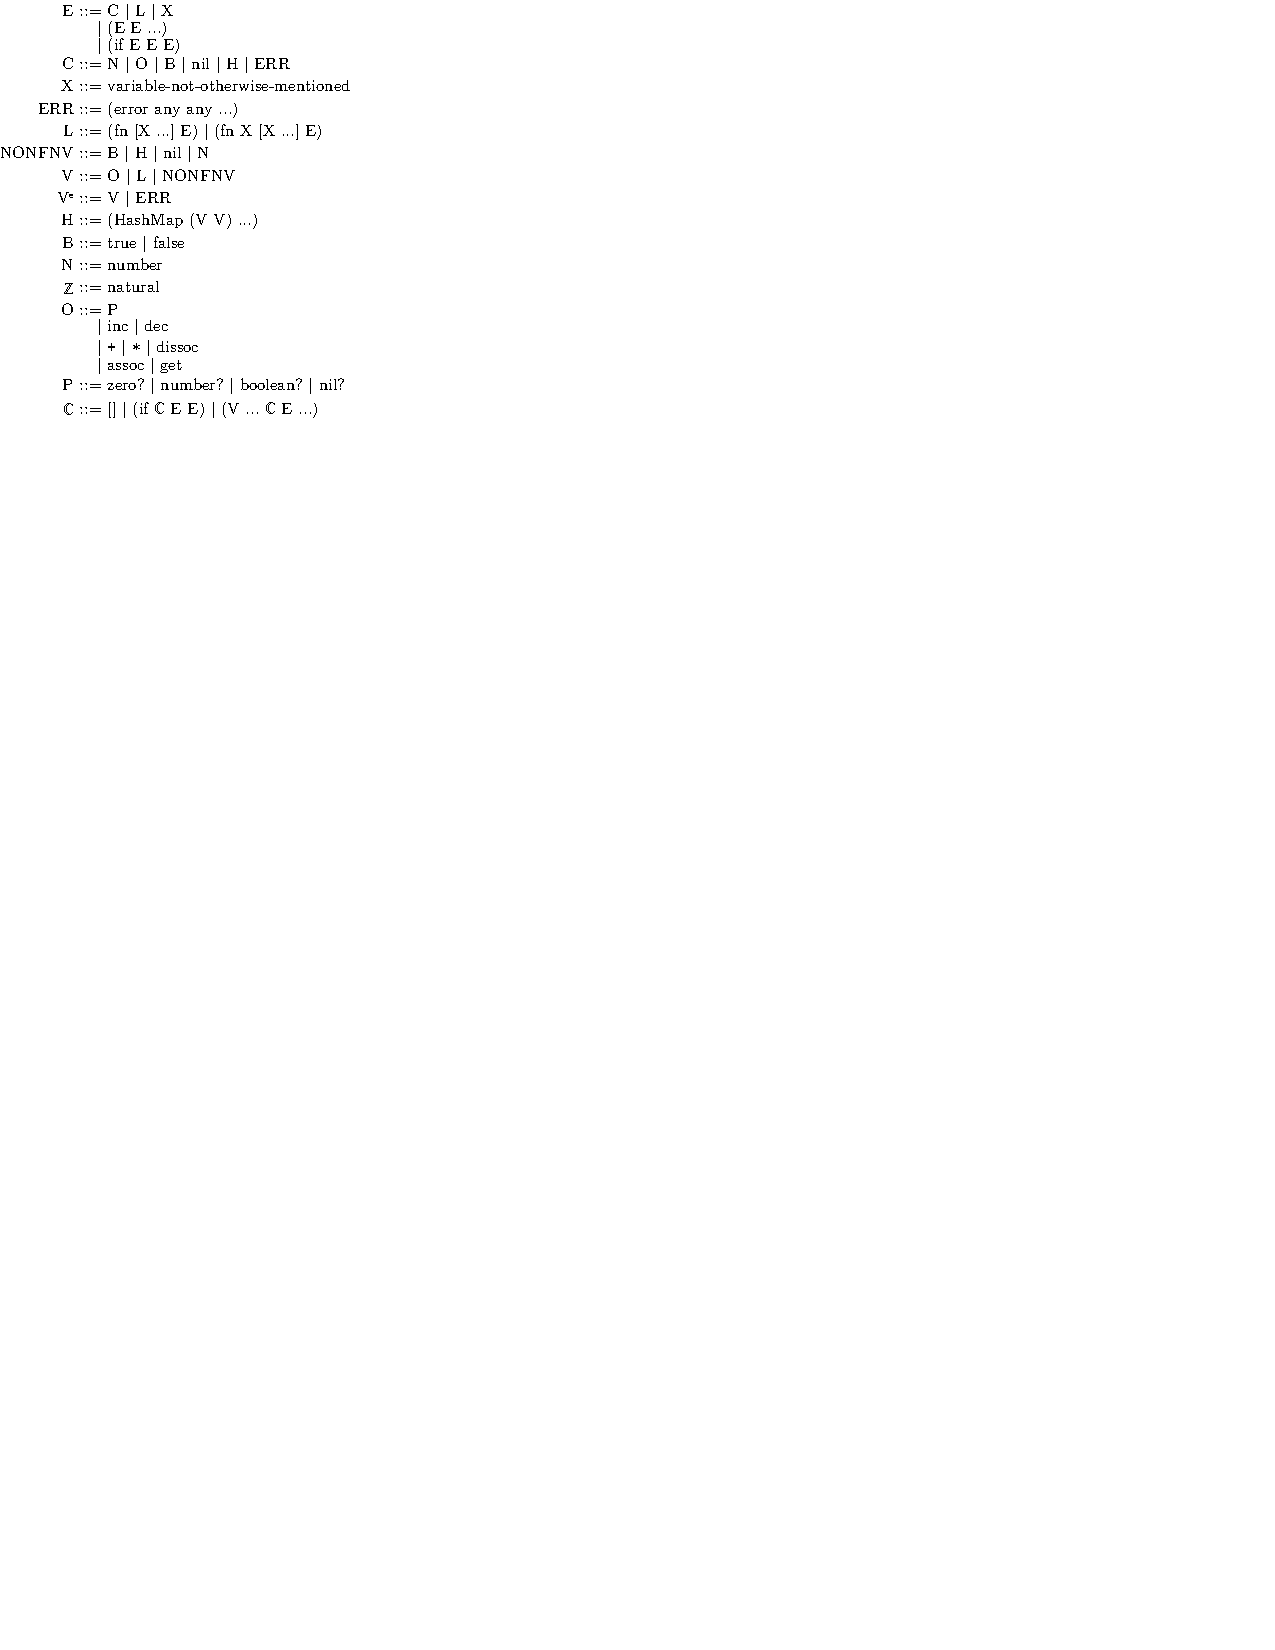
\includegraphics[]{redex/clojure-grammar.pdf}
\caption{Syntax of Terms in $\lambda c$.
  Expressions \texttt{E} consist of ``constant'' expressions \texttt{C}
  (numbers, built-in functions, booleans, nil, hash maps, and errors), 
  functions \texttt{L} (non-recursive, and recursive), variables, applications,
  and conditionals.
  Values are denoted \texttt{V}.
  }
\end{figure*}

%\begin{figure*}
$$
\begin{altgrammar}
  \e{} &::=& ... \alt &\mbox{Expressions} \\
\end{altgrammar}
$$
\caption{Syntax of $\lambda c_s$ (extending $\lambda c$)}
\end{figure*}


\begin{figure*}
  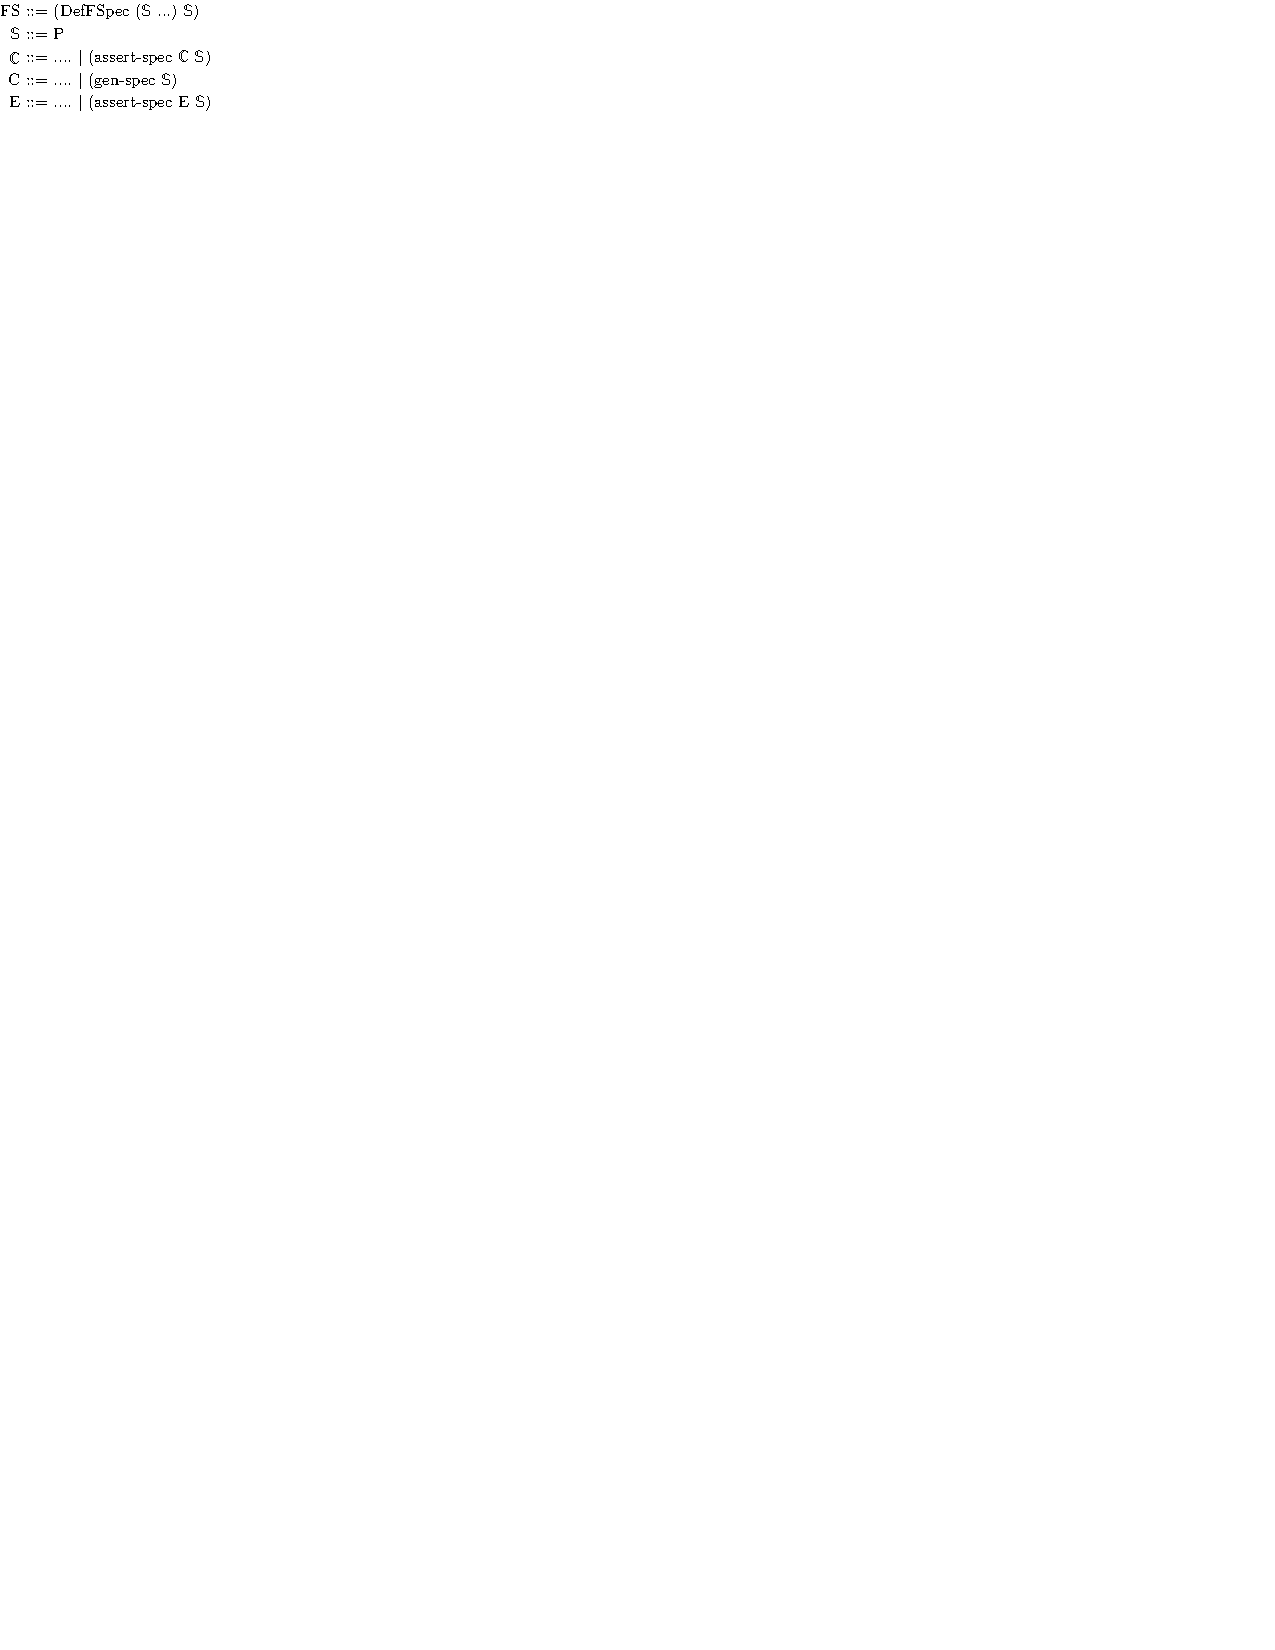
\includegraphics[]{redex/clojurespec-grammar.pdf}
\caption{Syntax of $\lambda c_s$ (extending $\lambda c$).
  We add the \texttt{assert-spec} form that takes an expression and a spec
  and checks the expression evaluates to a value conforming to the spec.
  We restrict specs to just predicates \texttt{P}.}
\end{figure*}

%\begin{figure*}
$$
\begin{altgrammar}
  \e{} &::=& ... \alt &\mbox{Expressions} \\
\end{altgrammar}
$$
\caption{Syntax of $\lambda c_s^f$ (extending $\lambda c_s$)}
\end{figure*}

\begin{figure*}
  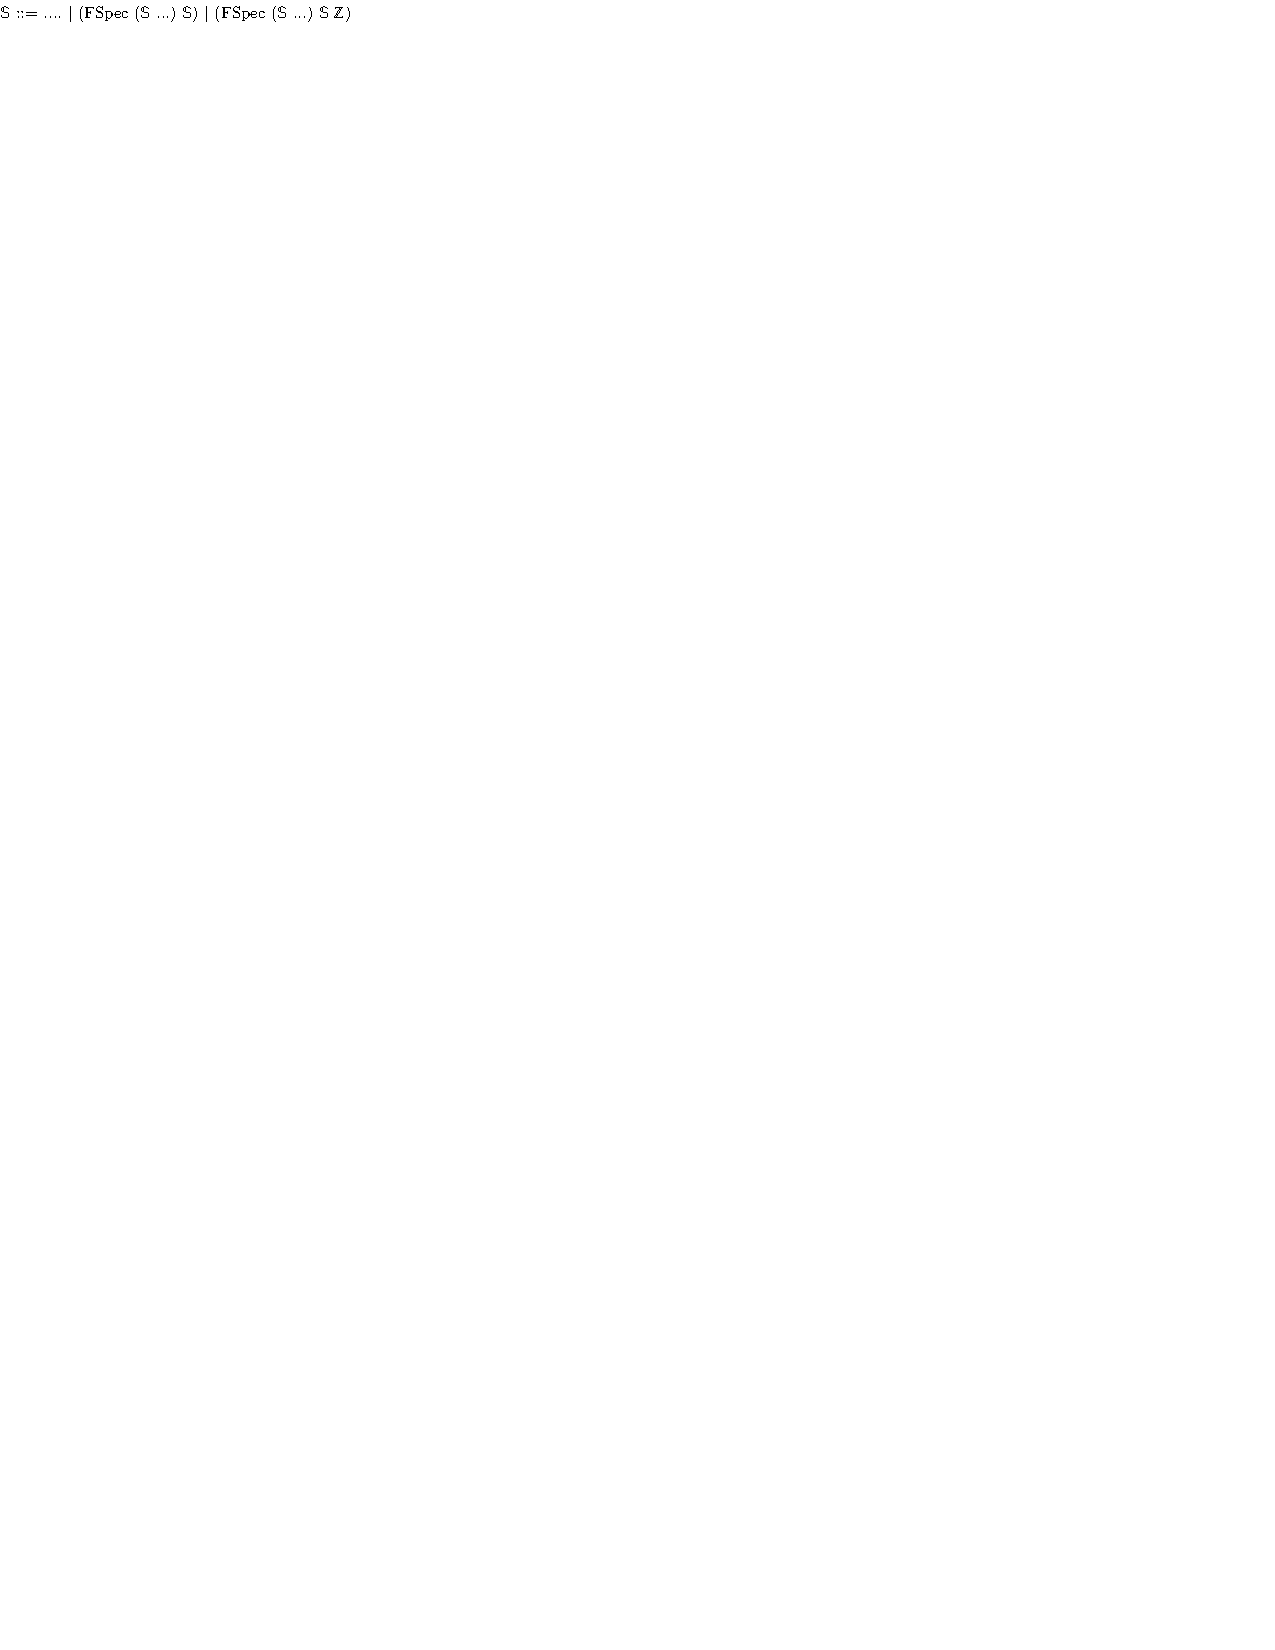
\includegraphics[]{redex/clojurespechof-grammar.pdf}
\caption{Syntax of $\lambda c_s^f$ (extending $\lambda c_s$).
  We add two forms of \texttt{fspec}s---the natural number represents how
  many times to generatively test a function value.
  }
\end{figure*}

\begin{figure}
  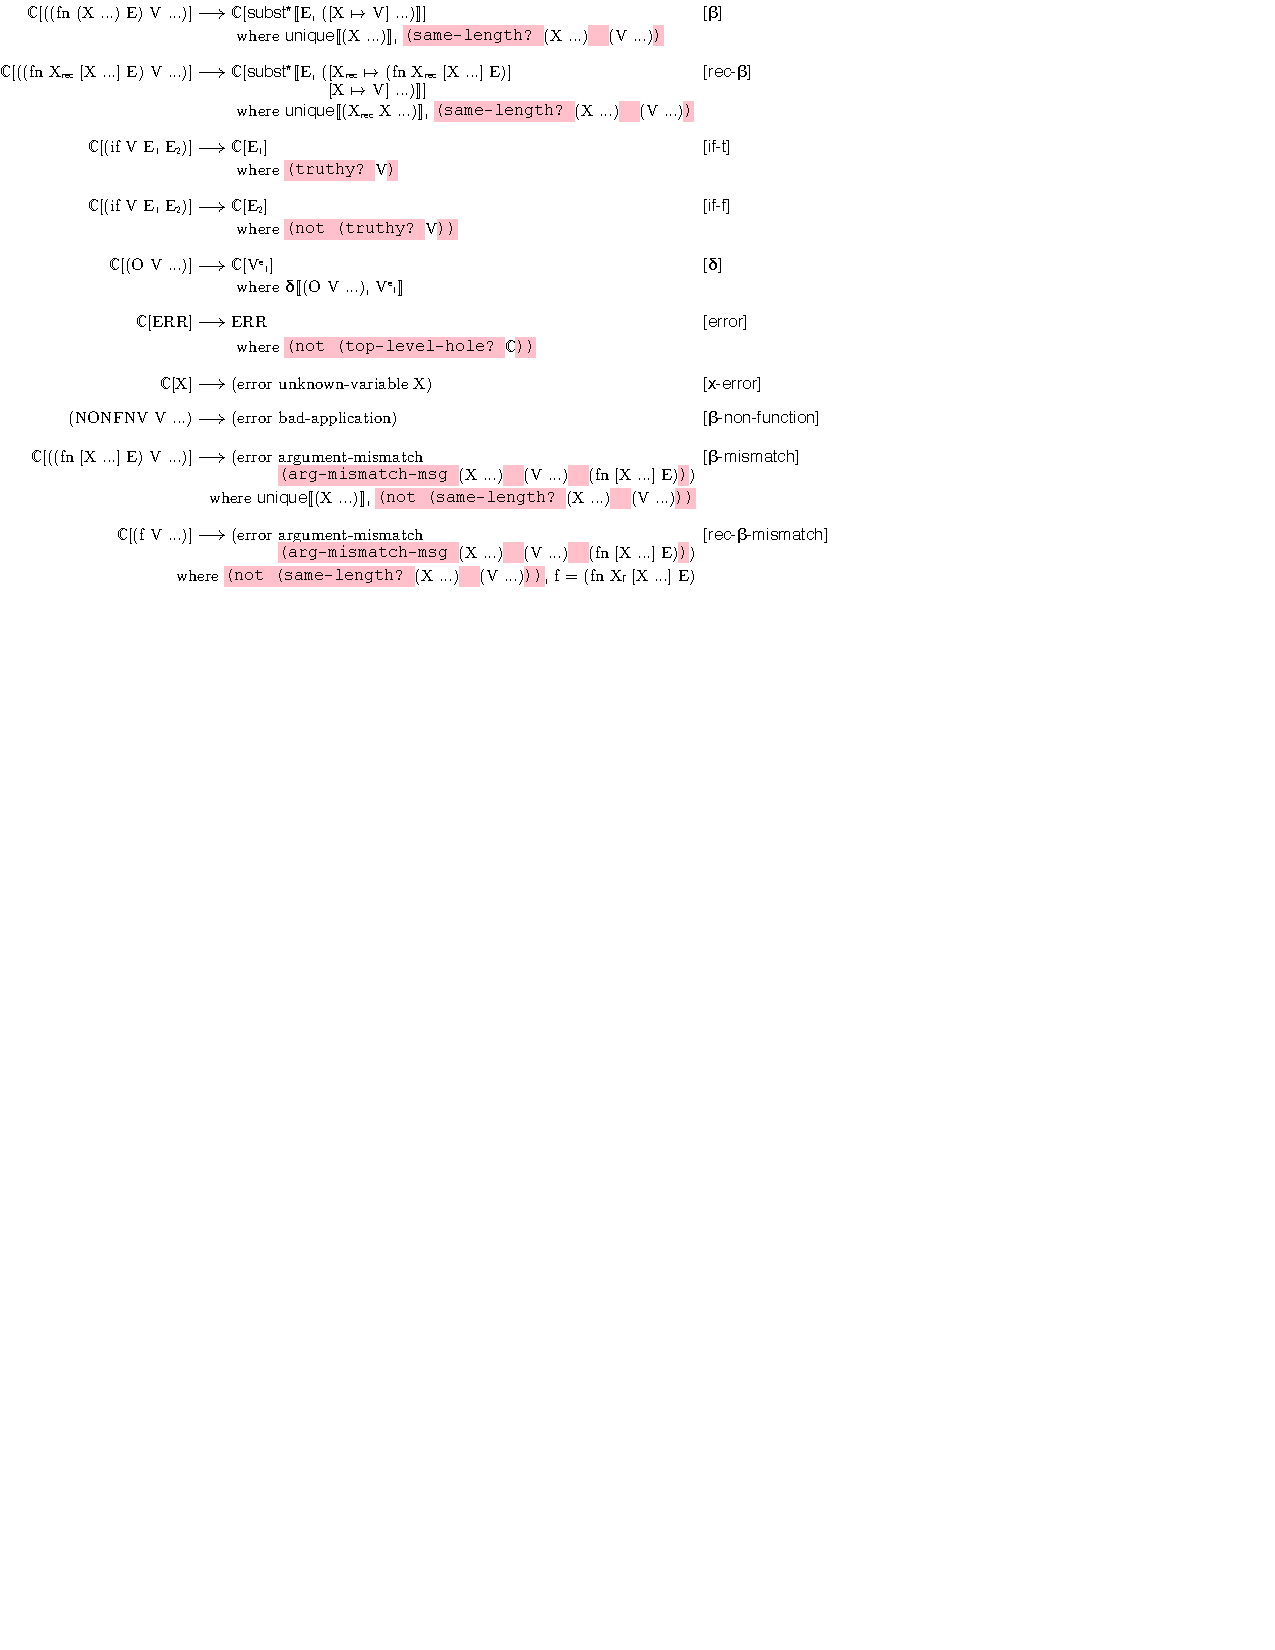
\includegraphics[]{redex/arrowv.pdf}
\caption{Small-step reduction relation in $\lambda c$.
  We define $\beta$ reduction rules for both types of functions.
  Then branching rules for conditionals (\texttt{false} and \texttt{nil} are false values),
  and constant functions ($\delta$, full definition omitted).
  Finally several rules for throwing detailed runtime errors.
  }
\end{figure}

\begin{figure*}
  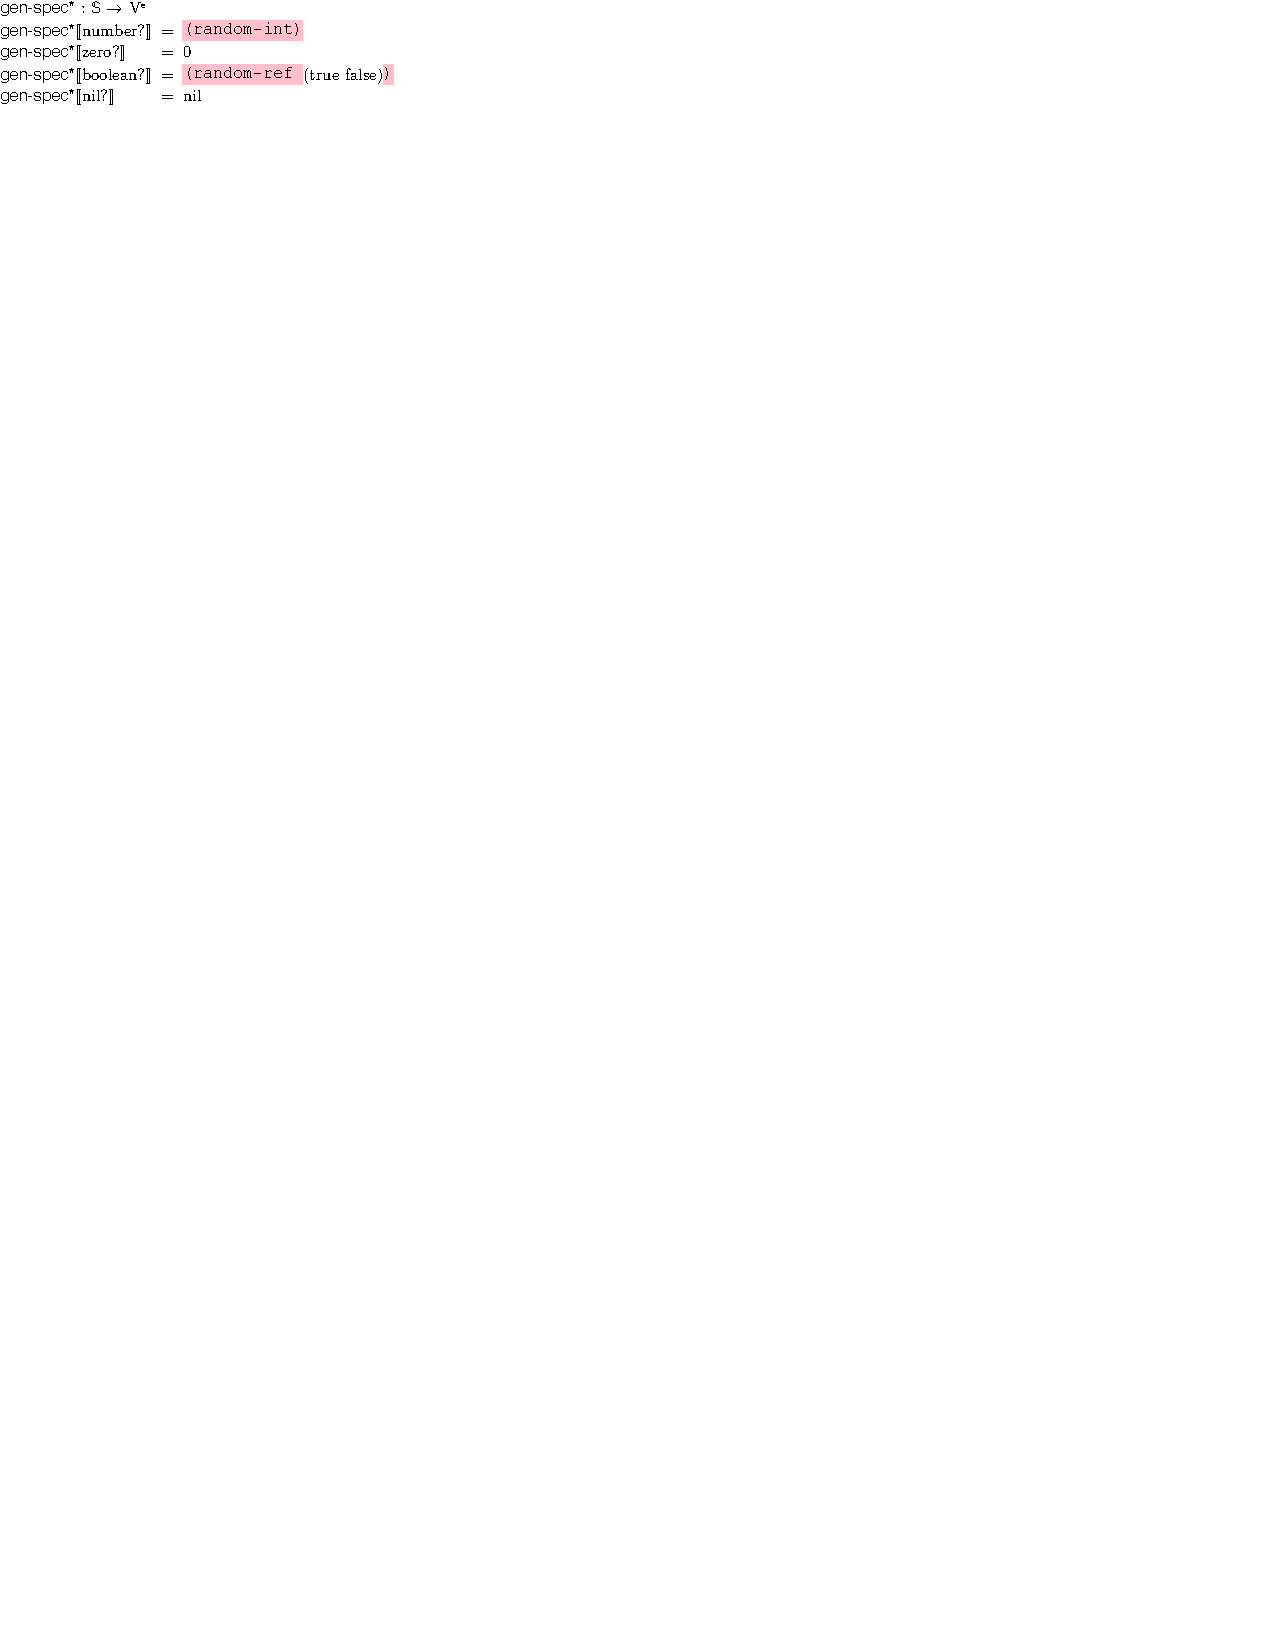
\includegraphics[]{redex/gen-spec*.pdf}

  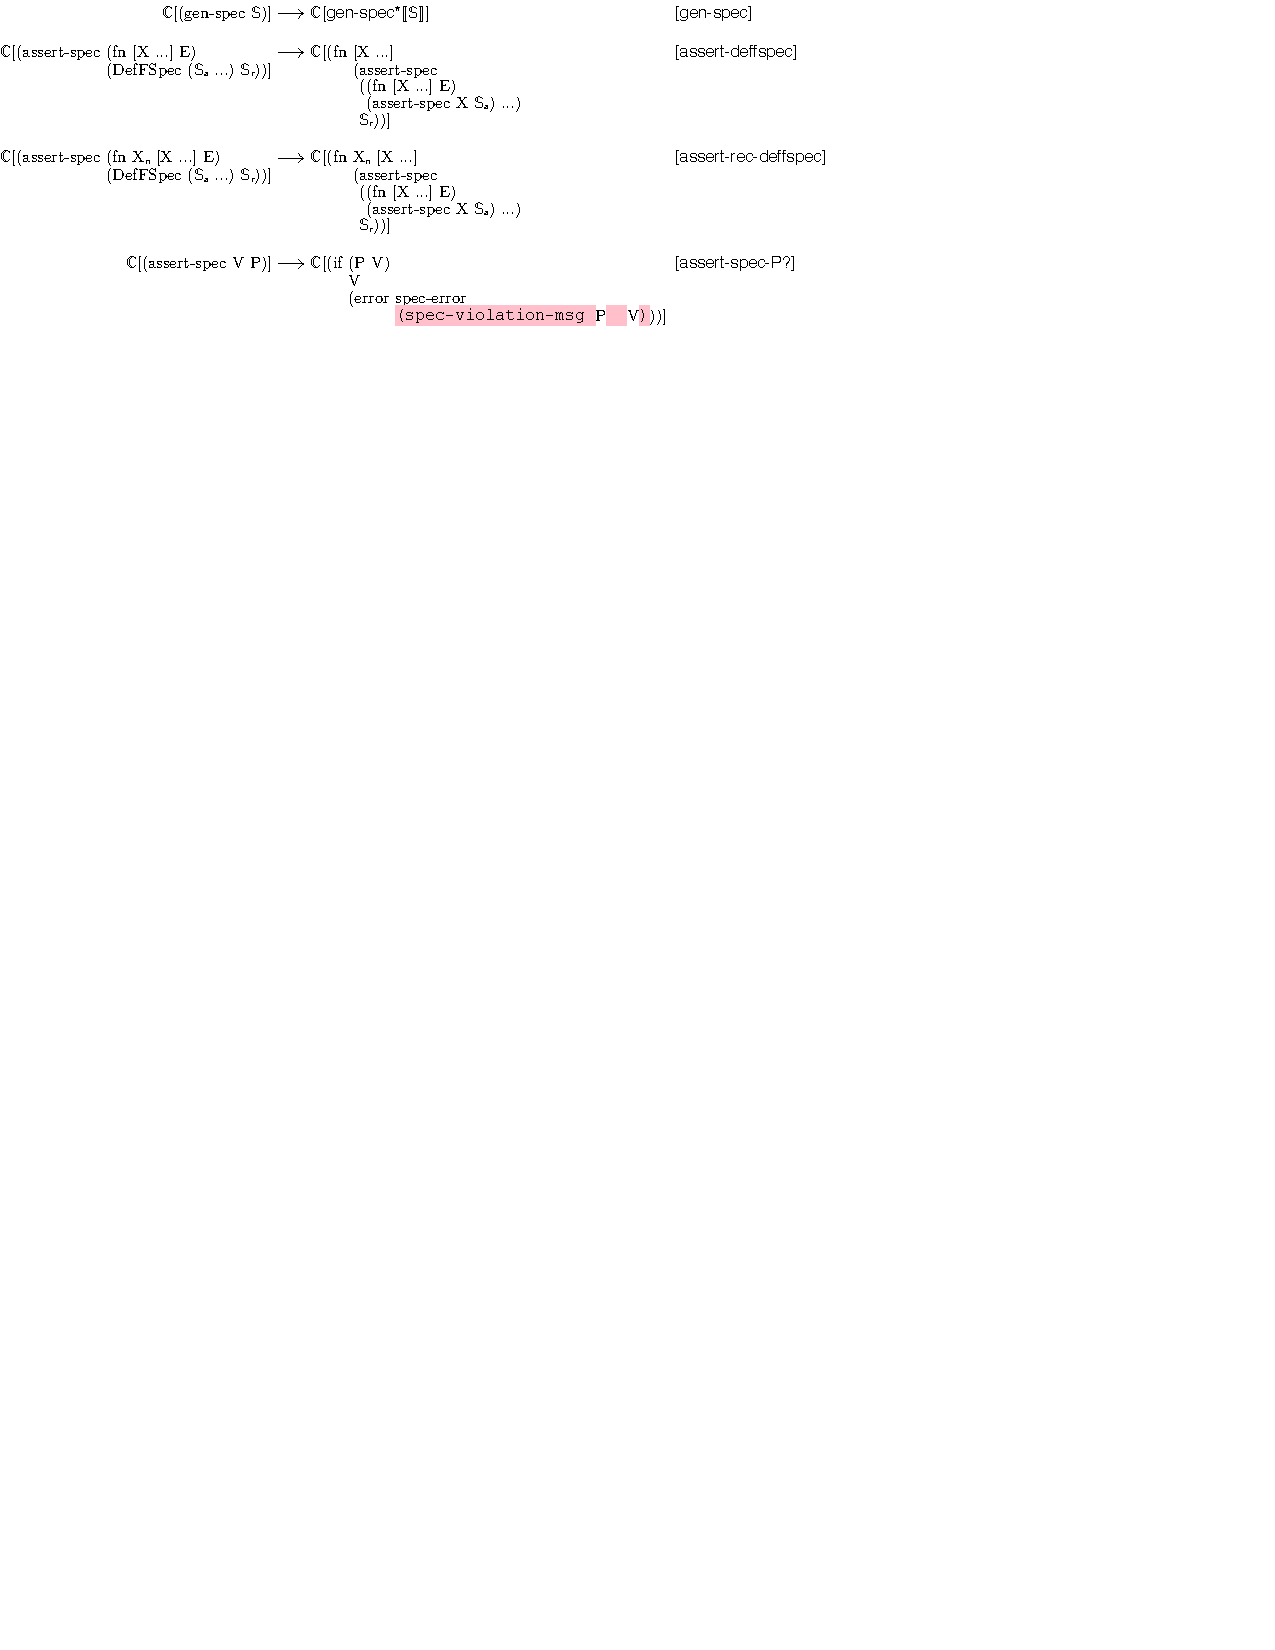
\includegraphics[]{redex/arrowvspec.pdf}
\caption{Small-step reduction relation in $\lambda c_s$ (extending $\lambda c$).
  \texttt{gen-spec} takes a spec and generates a value conforming to that spec
  via the \texttt{gen-spec*} metafunction.
  We define \texttt{assert-spec} with support for 
for \texttt{fdef} using traditional proxy checking semantics, and flat predicates.}
  \label{arrowvspec}
\end{figure*}

\begin{figure*}
  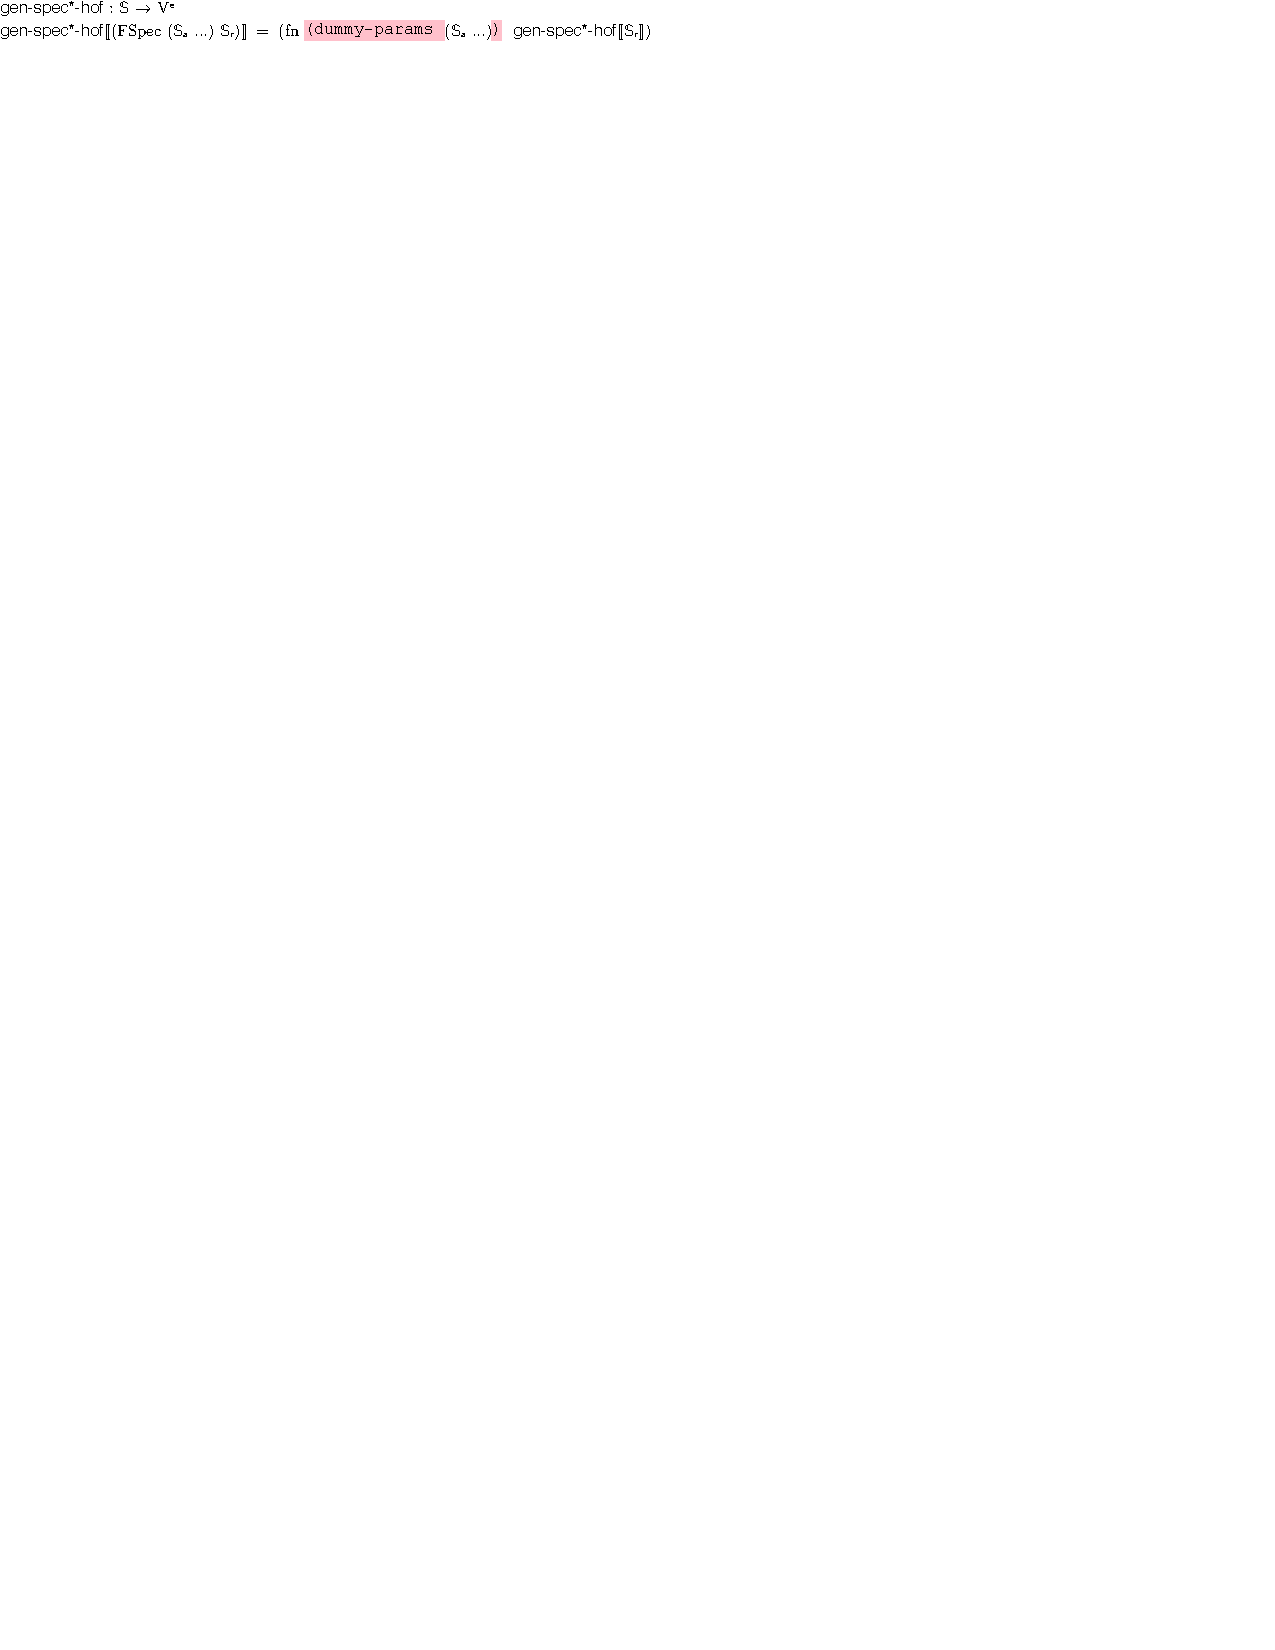
\includegraphics[]{redex/gen-spec*-hof.pdf}

  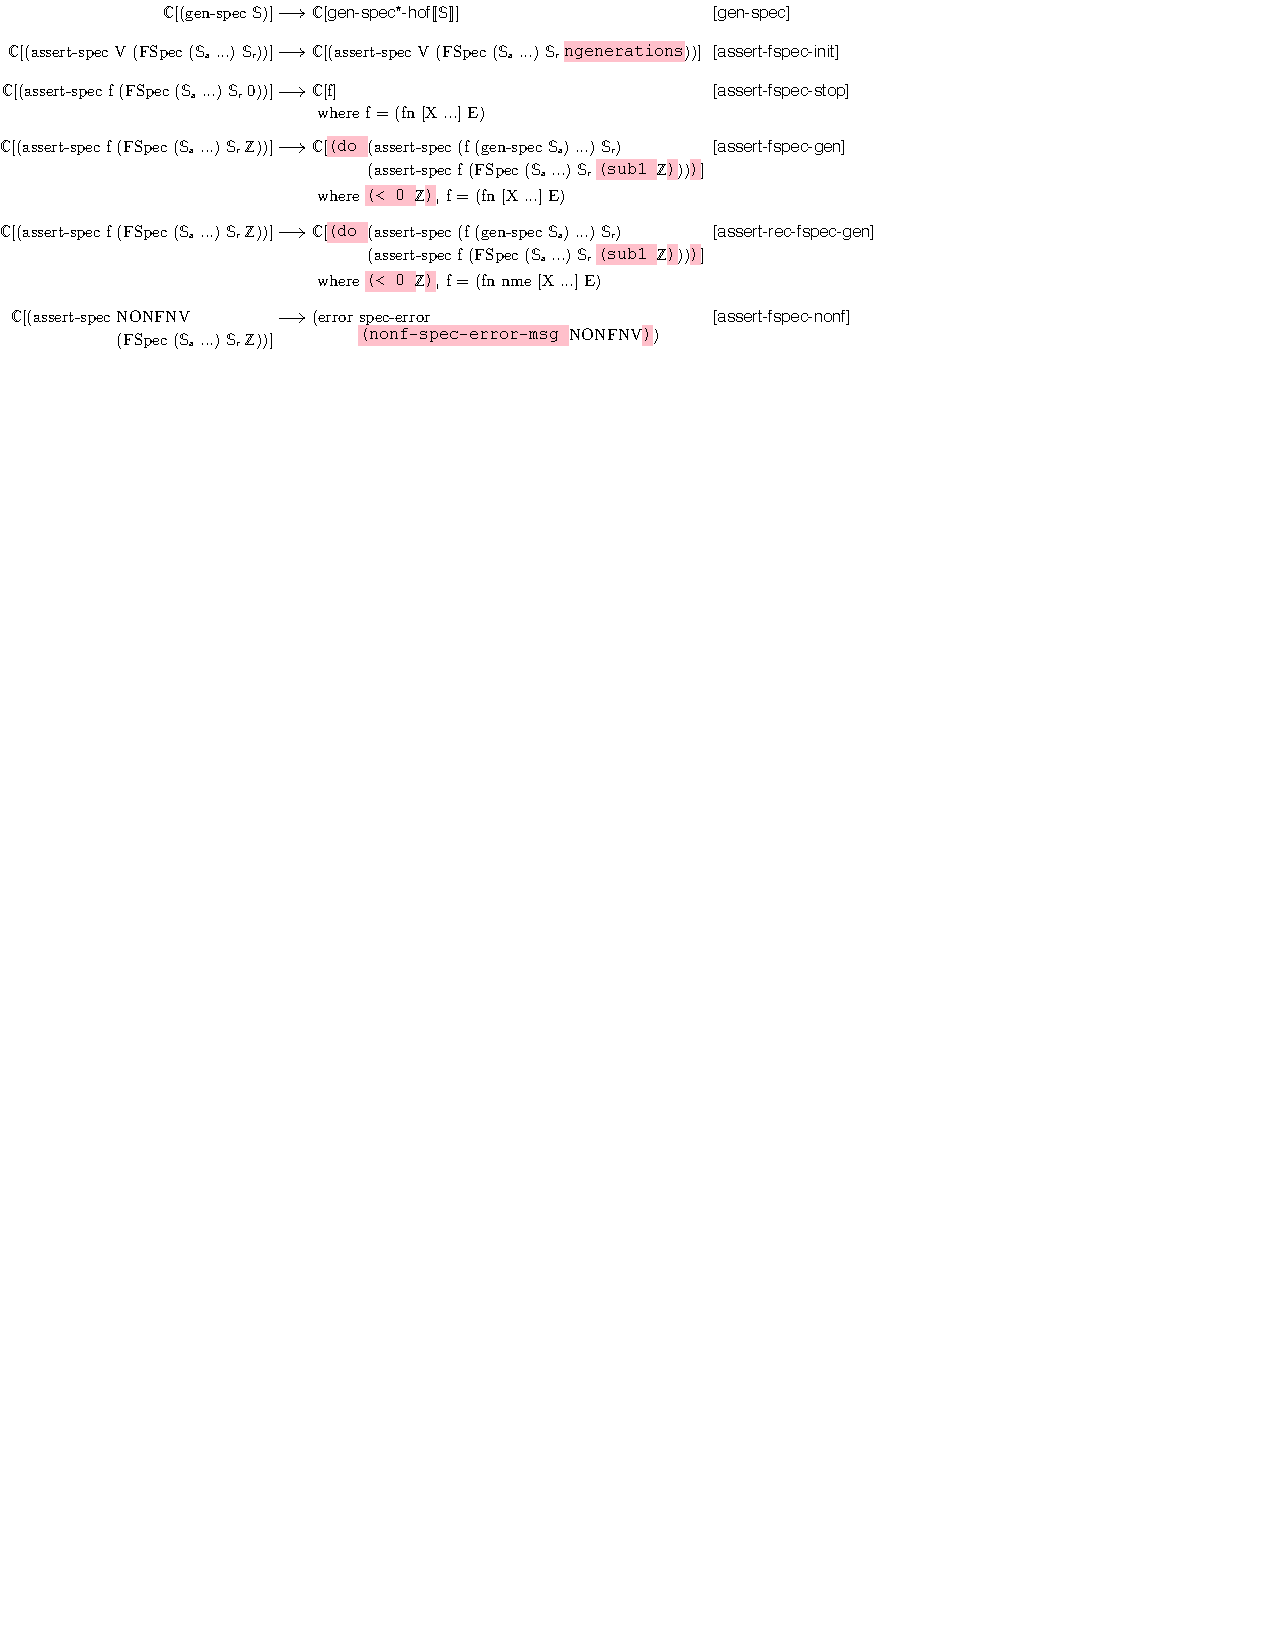
\includegraphics[]{redex/arrowvspec-hof.pdf}
  \caption{Small-step reduction relation for $\lambda c_{s}^{f}$ (extending $\lambda c_s$)
  \texttt{gen-spec} takes a spec and generates a value conforming to that spec
  via the \texttt{gen-spec*-hof} metafunction (which extends \texttt{gen-spec*} in Figure~\ref{arrowvspec}).
  }
\end{figure*}
